% !TeX root = RJwrapper.tex
\title{Residuals and Diagnostics for Ordinal Regression Models: An Introduction to the sure package}
\author{by Brandon M. Greenwell, Andrew J. McCarthy, Bradley C. Boehmke, and Dungang Liu}

\maketitle

\abstract{
Residual diagnostics is an important topic in the classroom, but it is less often used in practice. Part of the reason for this is that more complex models, like cumulative link models and logistic regression, do not produce standard residuals that are easily interpreted as those in ordinary linear regression. In this paper, we introduce the concept of surrogate residuals and demonstrate their use through the R package \pkg{sure}.
}


%%%%%%%%%%%%%%%%%%%%%%%%%%%%%%%%%%%%%%%%%%%%%%%%%%%%%%%%%%%%%%%%%%%%%%%%%%%%%%%%
\section{Introduction}
%%%%%%%%%%%%%%%%%%%%%%%%%%%%%%%%%%%%%%%%%%%%%%%%%%%%%%%%%%%%%%%%%%%%%%%%%%%%%%%%

Categorical outcomes are encountered frequently in practice across different fields. For example, in medical studies, the outcome of interest is often binary (e.g., presence or absence of a particular disease after applying a treatment). It is also relatively common for a categorical outcome to have a natural ordering. For instance, in an opinion poll, the response may be satisfaction, with categories low, medium, and high. In this case, the response is ordered: low $<$ medium $<$ high.

% Logistic and probit regression are popular choices for modelling a binary outcome. The surrogate approach to constructing residuals actually applies to a wide class of general models of the form 
% \begin{equation*}
%   \mathcal{Y} \sim F_a\left(y; \boldsymbol{X}, \boldsymbol{\beta}\right)
% \end{equation*}
% where $F_a\left(\cdot\right)$ is a discrete cumulative distribution function. This includes binary regression as a special case. For example, the probit model has
% \begin{equation*}
%   \mathcal{Y} \sim bernoulli\left[\Phi\left(\boldsymbol{x}^\top\boldsymbol{\beta}\right)\right],
% \end{equation*}
% where $\Phi\left(\cdot\right)$ is the cumulative distribution function for the standard normal distribution.

The \dfn{cumulative link} model is a natural choice for modelling an ordinal outcome. Consider an ordinal categorical outcome $\mathcal{Y}$ with ordered categories $1 < 2 < \dots < J$. In a cumulative link model, the cumulative probabilities are linked to the linear predictor according to
\begin{equation}
\label{eqn:clm}
  G^{-1}\left(\Pr\left\{\mathcal{Y} \le j\right\}\right) = \alpha_j + f\left(\boldsymbol{X}, \boldsymbol{\beta}\right),
\end{equation}
where $G$ is a continuous cumulative distribution function, $\alpha_j$ are the category-specific intercepts, $\boldsymbol{X}$ is a matrix of covariates, and $\boldsymbol{\beta}$ is a vector of fixed regression coefficients. The intercept parameters satisfy $-\infty = \alpha_0 < \alpha_1 < \dots < \alpha_{J-1} < \alpha_J = \infty$. We should point out that some authors (and software) use the alternate formulation
\begin{equation}
\label{eqn:clm2}
  G^{-1}\left(\Pr\left\{\mathcal{Y} \ge j\right\}\right) = \alpha_j^\star + f\left(\boldsymbol{X}, \boldsymbol{\beta}^\star\right),
\end{equation}
This formulation provides coefficients that are consistent with the ordinary logistic regression model. The estimated coefficients from model~\eqref{eqn:clm2} will have the opposite sign as those in model~\eqref{eqn:clm}.

Another way to interpret the cumulative link model is through a \dfn{latent} continuous random variable $\mathcal{Z} = -f\left(\boldsymbol{X}, \boldsymbol{\beta}\right) + \epsilon$, where $\epsilon$ is a continuous random variable with location parameter $0$, scale parameter $1$, and cumulative distribution function $G\left(\cdot\right)$. We then construct an ordered factor according to the rule
\begin{equation*}
  y = j \quad if \quad \alpha_{j - 1} < z \le \alpha_j.
\end{equation*}
For $\epsilon \sim N\left(0, 1\right)$, this leads to the usual probit model for ordinal responses,
\begin{equation*}
  \Pr\left\{\mathcal{Y} \le j\right\} = \Pr\left\{\mathcal{Z} \le \alpha_j\right\} = \Pr\left\{-f\left(\boldsymbol{X}, \boldsymbol{\beta}\right) + \epsilon \le \alpha_j\right\} = \Phi\left(\alpha_j + f\left(\boldsymbol{X}, \boldsymbol{\beta}\right)\right).
\end{equation*}
Common choices for the link function $G^{-1}\left(\cdot\right)$ and the implied (standard) distribution for $\epsilon$ are described in Table~\ref{tab:common}.
\begin{table}[!htbp]
  \begin{tabular}{llll}
    \toprule
      Link & Distribution of $\epsilon$ & $G\left(y\right)$ & $G^{-1}\left(p\right)$ \\
      \midrule
      logit\footnote{This is typically the default link function used by most statistical software.}   & logistic  & $\exp\left(y\right) / \left[1 + \exp\left(y\right)\right]$ & $\log\left[p / \left(1 - p\right)\right]$ \\
      probit & standard normal & $\Phi\left(y\right)$ & $\Phi^{-1}\left(p\right)$ \\
      log-log & Gumbel (max) & $\exp\left[-\exp\left(-y\right)\right]$ & $-\log\left[-\log\left(p\right)\right]$ \\
      complementary log-log & Gumbel (min) & $1 - \exp\left[-\exp\left(y\right)\right]$ & $\log\left[-\log\left(1 - p\right)\right]$ \\
      cauchit & Cauchy & $\pi^{-1} \arctan\left(y\right) + 1/2$ & $\tan\left(\pi p - \pi / 2\right)$ \\
      \bottomrule
  \end{tabular}
  \caption{Common link functions.}
  \label{tab:common}
\end{table}

There are a number of R packages that can be used to fit cumulative link models \eqref{eqn:clm} and \eqref{eqn:clm2}. The recommended package \CRANpkg{MASS} \citep{pkg-MASS} contains the function \code{polr} (proportional odds logistic regression) which, despite the name, can be used with all of the link functions described in Table~\ref{tab:common}. The \CRANpkg{VGAM} package \citep{pkg-VGAM} has the \code{vglm} function for fitting vector generalized linear models, which includes the broad class of cumulative link models. By default, \code{vglm} uses the same parameterization as in Equation~\eqref{eqn:clm}, but provides the option for using the parameterization seen in Equation~\eqref{eqn:clm2} as well; this will result in the estimated coefficients having the opposite sign. Package \CRANpkg{ordinal} \citep{pkg-ordinal} has the \code{clm} function for fitting cumulative link models. The popular \CRANpkg{rms} package \citep{pkg-rms} has two functions: \code{lrm} for fitting logistic regression and cumulative link models using the logit link, and \code{orm} for fitting ordinal regression models. Both of these functions use the parameterization seen in Equation~\eqref{eqn:clm2}.

For a continuous outcome $\mathcal{Y}$, the residual is traditionally defined as the difference between the observed and fitted values. For ordinal outcomes, the residuals are more difficult to define, and few definitions have been proposed in the literature. \citet{graphical-liu-2009} proposed using the cumulative sums of residuals derived from collapsing the ordered categories into multiple binary outcomes. Unfortunately, this method leads to multiple residuals for the ordinal outcome and therefore is difficult to interpret. \citet{residuals-li-2012} showed that the sign-based statistic (SBS)
\begin{equation}
\label{eqn:pres}
  R_{SBS} = E\left\{sign\left(y - \mathcal{Y}\right)\right\} = Pr\left\{y > \mathcal{Y}\right\} - Pr\left\{y < \mathcal{Y}\right\},
\end{equation}
can be used as a residual for proportional odds regression models; these are referred to later by \citeauthor{residuals-li-2012} as \dfn{probability-based residuals}, but we will follow \citet{residuals-liu-2017} and refer to them as SBS residuals. For an overview of the theoretical and graphical properties of the SBS residual \eqref{eqn:pres}, see \citet{residuals-liu-2017}. These are available in the \CRANpkg{PResiduals} package \citep{pkg-PResiduals}. A limitation with the SBS residuals is that they are based on a discrete outcome and hence, are discrete themselves. This makes using them in various diagnostic plots far less useful, as will be illustrated.


%%%%%%%%%%%%%%%%%%%%%%%%%%%%%%%%%%%%%%%%%%%%%%%%%%%%%%%%%%%%%%%%%%%%%%%%%%%%%%%%
\section{Surrogate-based residuals}
\label{sec:surrogate}
%%%%%%%%%%%%%%%%%%%%%%%%%%%%%%%%%%%%%%%%%%%%%%%%%%%%%%%%%%%%%%%%%%%%%%%%%%%%%%%%

\citet{residuals-liu-2017} propose a new type of residual that is based on a continuous variable $S$ that acts as a surrogate for the ordinal outcome $\mathcal{Y}$. This surrogate residual is defined as
\begin{equation}
\label{eqn:sure}
R_S = S - E\left(S | \boldsymbol{X}\right),
\end{equation}
where $S$ is a continuous variable based on the conditional distribution of the latent variable $\mathcal{Z}$ given $\mathcal{Y}$. In particular, given $\mathcal{Y} = y$, \citet{residuals-liu-2017} show that $S$ follows a truncated distribution obtained by truncating the distribution of $\mathcal{Z} = -f\left(\boldsymbol{X}, \boldsymbol{\beta}\right) + \epsilon$ using the interval $\left(\alpha_{y - 1}, \alpha_y\right)$. The benefit of the surrogate-based residual \eqref{eqn:sure} is that it is based on a continuous variable $S$, hence, $R_S$ is also continuous. 

Furthermore, it can be shown \citep{residuals-liu-2017} that if the hypothesized model agrees with the true model, then $R_S$ will have the following properties:
\begin{description}
  \item[symmetry around zero] $E\left(R_S | \boldsymbol{X}\right) = 0$;
  \item[homogeneity] $Var\left(R_S | \boldsymbol{X}\right) = c$, a constant that is independent of $\boldsymbol{X}$;
  \item[reference distribution] the empirical distribution of $R_S$ approximates an explicit distribution that is related to the link function $G^{-1}\left(\cdot\right)$.
\end{description}
These properties allow for a thorough examination of the residuals to check model adequacy and misspecification of the mean structure and link function.


%%%%%%%%%%%%%%%%%%%%%%%%%%%%%%%%%%%%%%%%%%%%%%%%%%%%%%%%%%%%%%%%%%%%%%%%%%%%%%%%
\subsection{Jittering for general models}
\label{sec:jittering}
%%%%%%%%%%%%%%%%%%%%%%%%%%%%%%%%%%%%%%%%%%%%%%%%%%%%%%%%%%%%%%%%%%%%%%%%%%%%%%%%

The latent method discussed in Section~\ref{sec:surrogate} applies to cumulative link models for ordinal outcomes. For more general models, we can define a surrogate using a technique called \dfn{jittering}. Suppose the true model for an ordinal outcome $\mathcal{Y}$
\begin{equation}
  \mathcal{Y} \sim F_a\left(y; \boldsymbol{X}, \boldsymbol{\beta}\right),
\end{equation}
where $F\left(\cdot\right)$ is a discrete cumulative distribution function. This model is general enough to cover the cumulative link models \eqref{eqn:clm} and \eqref{eqn:clm2}, and nearly any parametric or nonparametric model for ordinal outcomes.

\citet{residuals-liu-2017} suggest defining the surrogate $S$ using either of the following two approaches:
\begin{enumerate}
  \item jittering on the outcome scale: $S | \mathcal{Y} = y \sim \mathcal{U}\left[y, y + 1\right]$;
  \item jittering on the probability scale: $S | \mathcal{Y} = y \sim \mathcal{U}\left[F_a\left(y - 1\right), F_a\left(y\right)\right]$.
\end{enumerate}
Once a surrogate is obtained, we define the surrogate residuals in the same way as Equation~\eqref{eqn:sure}.
In either case, if the hypothesized model is correct, then symmetry around zero still holds; that is $E\left(R_S | \boldsymbol{X}\right) = 0$. For the latter case, if the hypothesized model is correct then $R_S | \boldsymbol{X} \sim \mathcal{U}\left(-1/2, 1/2\right)$. In other words, jittering on the probability scale has the additional property that the conditional distribution of $R_S$ given $\boldsymbol{X}$ has an explicit form. This allows for a full examination of the distributional information of the residual.


%%%%%%%%%%%%%%%%%%%%%%%%%%%%%%%%%%%%%%%%%%%%%%%%%%%%%%%%%%%%%%%%%%%%%%%%%%%%%%%%
\subsection{Bootstrapping}
%%%%%%%%%%%%%%%%%%%%%%%%%%%%%%%%%%%%%%%%%%%%%%%%%%%%%%%%%%%%%%%%%%%%%%%%%%%%%%%%

Since the surrogate residuals are based on random sampling, additional error is introduced. One way to minimize this sampling error and help stabilize any patterns in diagnostic plots is to use the bootstrap \citep{efron-another-1979}.

The procedure for bootstrapping surrogate residuals is similar to the model-based bootstrap algorithm used in linear regression. To obtain the $b$-th bootstrap replicate of the residuals, \citet{residuals-liu-2017} suggest the following algorithm:
\begin{description}
  \item[Step 1] Perform a standard case-wise bootstrap of the original data to obtain the bootstrap sample $\left\{\left(\boldsymbol{X}_{1b}^\star, \mathcal{Y}_{1b}^\star\right), \dots, \left(\boldsymbol{X}_{ nk}^\star, \mathcal{Y}_{nk}^\star\right)\right\}$.
  \item[Step 2] Using the procedure outlined in the previous section, obtain a sample of surrogate residuals $R_{S_{1b}}^\star, \dots, R_{S_{nb}}^\star$ using the bootstrapped data obtained in \textbf{Step 1}.
\end{description}

This procedure is repeated a total of $B$ times. For residual vs. covariate (i.e., $R$ vs. $X$) plots and residual vs. fitted value (i.e., $R$ vs. $f\left(\boldsymbol{X}, \boldsymbol{\beta}\right)$) plots, we simply scatter all $B \times n$ residuals on the same plot. This approach is valid since the bootstrap samples are drawn independently from each other. For large data sets, we find it useful to also lower the opacity of the data points to help alleviate any issues with over plotting. For Q-Q plots, on the other hand, \citet{residuals-liu-2017} suggest using the median of the $B$ bootstrap distributions which is the implementation used in the \CRANpkg{sure} package \citep{pkg-sure}.


%%%%%%%%%%%%%%%%%%%%%%%%%%%%%%%%%%%%%%%%%%%%%%%%%%%%%%%%%%%%%%%%%%%%%%%%%%%%%%%%
\section{Surrogate-based residuals in R}
%%%%%%%%%%%%%%%%%%%%%%%%%%%%%%%%%%%%%%%%%%%%%%%%%%%%%%%%%%%%%%%%%%%%%%%%%%%%%%%%

The \pkg{sure} package supports a variety of R packages for fitting cumulative link and other types of models. The supported packages and their corresponding functions are described in Table~\ref{tab:pkgs}.
\begin{table}[!htbp]
  \centering
  \begin{tabular}{llll}
    \toprule
      Package & Function(s) & Model & Parameterization \\
      \midrule
      \pkg{stats}   & \code{glm}  & binary regression   & NA \\
      \pkg{MASS}    & \code{polr} & cumulative link     & $Pr\left\{\mathcal{Y} \le j\right\}$ \\
      \pkg{rms}     & \code{lrm}  & cumulative link     & $Pr\left\{\mathcal{Y} \ge j\right\}$ \\
                    & \code{lrm}  & logistic regression & NA \\
                    & \code{orm}  & cumulative link     & $Pr\left\{\mathcal{Y} \ge j\right\}$ \\
      \pkg{ordinal} & \code{clm}  & cumulative link     & $Pr\left\{\mathcal{Y} \le j\right\}$ \\
      \pkg{VGAM}    & \code{vglm} & cumulative link     & $Pr\left\{\mathcal{Y} \le j\right\}$\footnote{This is the default parameterization used by \code{vglm}. This can be reversed by setting \code{reverse = TRUE}.} \\
                    & \code{vgam} & cumulative link     & $Pr\left\{\mathcal{Y} \le j\right\}$ \\
      \bottomrule
  \end{tabular}
  \caption{Ordinal regression modelling packages supported by \pkg{sure} and the corresponding parameterization they use for fitting cumulative link models.}
  \label{tab:pkgs}
\end{table}

The \pkg{sure} package currently only exports four functions:
\begin{itemize}
  \item \code{resids}---for constructing surrogate residuals;
  \item \code{surrogate}---for generating the surrogate response values used in the residuals;
  \item \code{autoplot}---produce various diagnostic plots using \CRANpkg{ggplot2} graphics \citep{pkg-ggplot2};
 \item \code{gof}---simulate p-values from a goodness-of-fit test.
\end{itemize}
In addition, the package also includes three simulated data sets: \code{df1}, \code{df2}, and \code{df3}. These data sets are used throughout the paper to demonstrate how the surrogate-based residual can be useful as a diagnostic tool for ordinal regression models.


%%%%%%%%%%%%%%%%%%%%%%%%%%%%%%%%%%%%%%%%%%%%%%%%%%%%%%%%%%%%%%%%%%%%%%%%%%%%%%%%
\subsection{Detecting a misspecified mean structure}
%%%%%%%%%%%%%%%%%%%%%%%%%%%%%%%%%%%%%%%%%%%%%%%%%%%%%%%%%%%%%%%%%%%%%%%%%%%%%%%%

For illustration, the data frame \code{df1} contains $n = 2000$ observations from the following cumulative link model:
\begin{equation}
\label{eqn:quadratic}
  Pr\left\{\mathcal{Y} \le j\right\} = \Phi\left(\alpha_j + \beta_1 X + \beta_2 X ^ 2\right), \quad j = 1, 2, 3, 4,
\end{equation}
where $\alpha_1 = -16$, $\alpha_2 = -12$, $\alpha_3 = -8$, $\beta_1 = 8$, $\beta_2 = -1$, and $X \sim \mathcal{U}\left(1, 7\right)$. These simulated data are available in the \code{df1} data frame from the \pkg{sure} package and are loaded automatically with the package; see \code{?df1} for details. Below, we fit a (correctly specified) probit model using the \code{polr} function from the \pkg{MASS} package.
\begin{example}
# Load required package(s)
library(MASS)

# Fit a cumulative link model with probit link
fit.polr <- polr(y ~ x + I(x ^ 2), data = df1, method = "probit")
\end{example}

The code chunk below obtains the SBS residuals \eqref{eqn:pres} from the previously fitted probit model \code{fit.polr} using the \pkg{PResiduals} package and constructs a couple of diagnostic plots. The results are displayed in Figure~\ref{fig:quadratic-correct-sbs}. 
\begin{example}
# Load required package(s)
library(PResiduals)

# Obtain the SBS/probability-scale residuals
pres <- presid(fit.polr)

# Residual vs. covariate plot
p1 <- ggplot(data.frame(x = df1$x, y = pres), aes(x, y)) +
  geom_point(alpha = 0.5) +
  geom_smooth(color = "red", se = FALSE) +
  ylab("Probability-scale residual")
  
# Q-Q plot of the residuals
p2 <- ggplot(data.frame(y = pres), aes(sample = y)) +
  stat_qq(distribution = qunif, dparams = list(min = -1, max = 1), alpha = 0.5) +
  xlab("Sample quantile") +
  ylab("Theoretical quantile")

# Figure 1
grid.arrange(p1, p2, ncol = 2)
\end{example}
(\strong{Note:} the reference distribution for the SBS residual is the $\mathcal{U}\left(-1, 1\right)$ distribution.) As can be seen in Figure~\ref{fig:quadratic-correct-sbs}, the SBS residuals, which are inherently discrete, often display unusual patterns in diagnostic plots, making them less useful as a diagnostic tool. There is a pattern for each of the $J = 4$ classes!
\begin{figure}[!htbp]
  \centering
  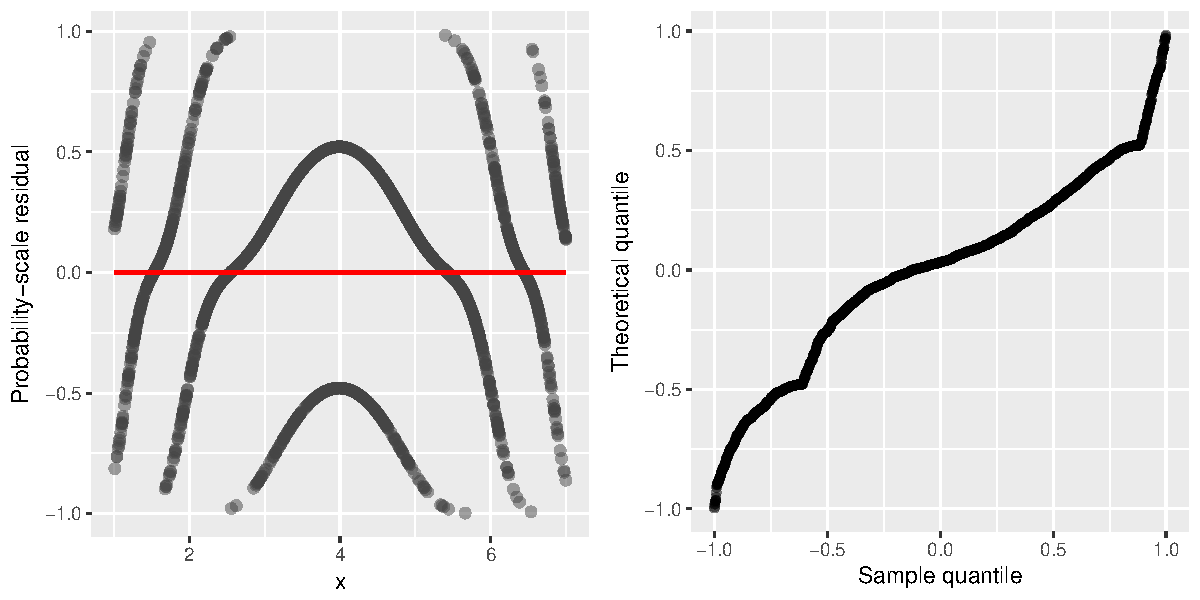
\includegraphics[width=1\textwidth]{quadratic-correct-sbs}
  \caption{SBS residual plots for the (correctly specified) probit model fit to the \code{df1} data set. \textit{Left}: Residual vs. covariate plot. \textit{Right}: Q-Q plot of the residuals. Nonparametric smooths are indicated by red curves.}
  \label{fig:quadratic-correct-sbs}
\end{figure}

Similarly, we can use the \code{resids} function in package \pkg{sure} to obtain the surrogate-based residuals discussed in Section~\ref{sec:surrogate}. This is illustrated in the following code chunk. the results are displayed in Figure~\ref{fig:quadratic-correct-surrogate}.
\begin{example}
# Load required package(s)
library(ggplot2)
library(sure)

# Obtain surrogate-based residuals
set.seed(101)  # for reproducibility
sres <- resids(fit.polr)

# Residual vs. covariate plot
p1 <- autoplot(sres, what = "covariate", x = df1$x, xlab = "x")

# Q-Q plot of the residuals
p2 <- autoplot(sres, what = "qq", distribution = pnorm)

# Figure ?
grid.arrange(p1, p2, ncol = 2)
\end{example}
\begin{figure}[!htbp]
  \centering
  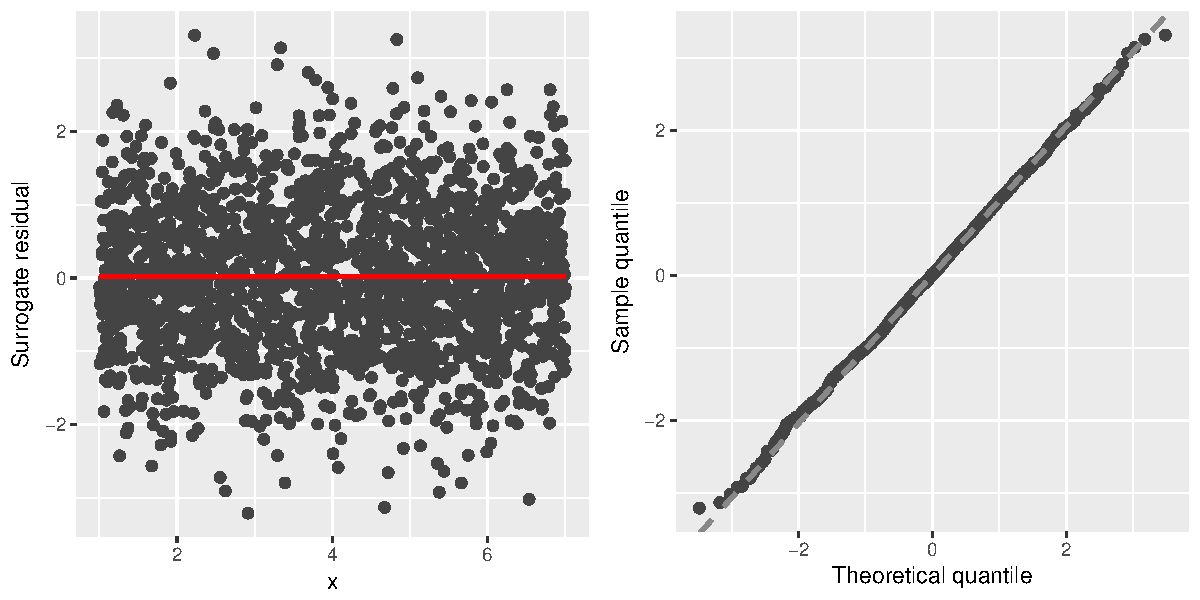
\includegraphics[width=1\textwidth]{quadratic-correct-surrogate}
  \caption{Surrogate-based residual plots for the (correctly specified) probit model fit to the \code{df1} data set. \textit{Left}: Residual vs. covariate plot. \textit{Right}: Q-Q plot of the residuals. Nonparametric smooths are indicated by red curves.}
  \label{fig:quadratic-correct-surrogate}
\end{figure}

The \pkg{sure} package also includes \code{autoplot} methods for the various classes of models listed in Table~\ref{tab:pkgs}, so you can just give \code{autoplot} the fitted model directly. The benefit of this approach is that the fitted values and reference distribution (used in Q-Q plots) are automatically extracted. For example, to reproduce the Q-Q plot in Figure~\ref{fig:quadratic-correct-surrogate}, we could have just used
\begin{example}
set.seed(101)  # for reproducibility
autoplot(fit.polr, what = "qq")  # same as top right of Figure 1
\end{example}

Suppose that we did not include the quadratic term in our fitted model. We would expect a residual-vs-$x$ plot to indicate that such a quadratic term is missing. Below we update the previously fitted model by removing the quadratic term, then update the residual-vs-covariate plots (code not shown). The updated residual plots are displayed in Figure~\ref{fig:quadratic}.
\begin{example}
fit.polr <- update(fit.polr, y ~ x)  # remove quadratic term
\end{example}
The SBS residuals gives some indication of a misspecified mean structure, but this only becomes more clear with increasing $J$, and the plot is still discrete. This is overcome by the surrogate residuals which produces a residual plot not unlike those seen in ordinary linear regression models.

\begin{figure}[!htbp]
  \centering
  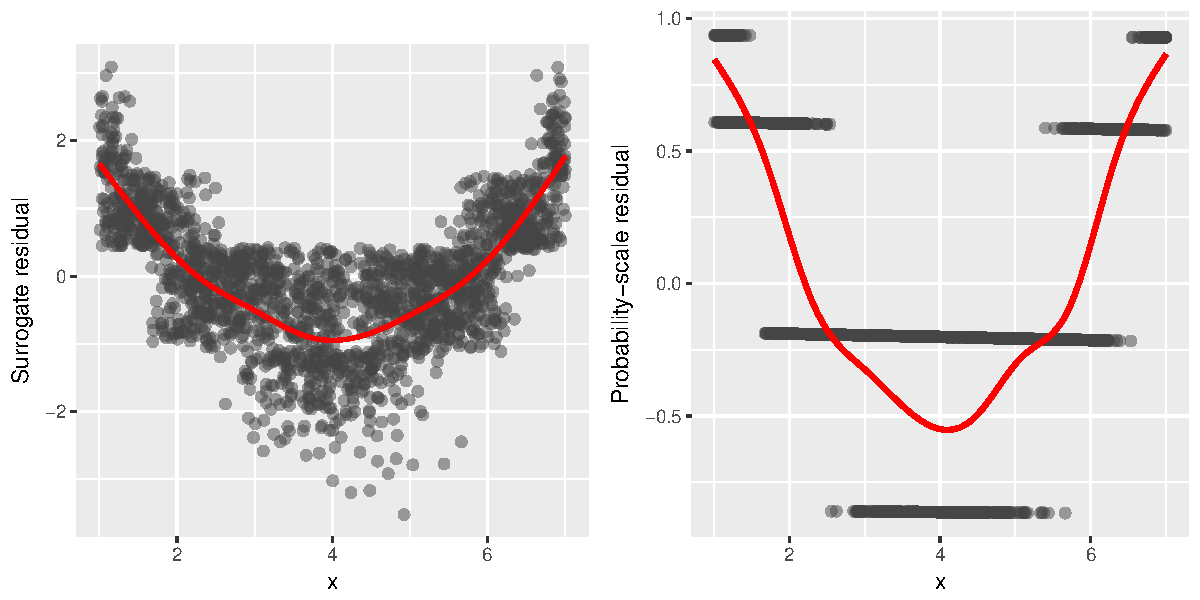
\includegraphics[width=1\textwidth]{quadratic}
  \caption{Residual-vs-covariate plots for a probit model with a misspecified mean structure fit to the simulated data from model \eqref{eqn:quadratic}. \textit{Left}: Surrogate residuals. \textit{Right}: SBS residuals. Nonparametric smooths are indicated by red curves.}
  \label{fig:quadratic}
\end{figure}


%%%%%%%%%%%%%%%%%%%%%%%%%%%%%%%%%%%%%%%%%%%%%%%%%%%%%%%%%%%%%%%%%%%%%%%%%%%%%%%%
\subsection{Detecting heteroscedasticty}
%%%%%%%%%%%%%%%%%%%%%%%%%%%%%%%%%%%%%%%%%%%%%%%%%%%%%%%%%%%%%%%%%%%%%%%%%%%%%%%%

One issue that often raises concerns in  statistical inference is that of heteroscedasticity; that is, when the error term has non constant variance. Heteroscedasticity can bias the statistical inference and lead to improper standard errors, confidence intervals, and $p$-values. Therefore, it is imperative to identify heteroscedacticity whenever present and take appropriate action (e.g., transformations, etc.). In ordinary linear regression, this topic has been covered extensively. For categorical models, on the other hand, not much has been proposed in the literature.

As discussed in Section~\ref{sec:surrogate}, one of the properties of the surrogate-based residual $R_S$ is that, if the model is specified correctly, then $Var\left(R_S | X\right) = c$, where $c$ is a constant.

For this example, we generated $n = 2000$ observations from the following ordered probit model:
\begin{equation*}
  Pr\left\{\mathcal{Y} \le j\right\} = \Phi\left\{\left(\alpha_j + \beta X\right) / \sigma_X\right\}, \quad j = 1, 2, 3, 4, 5,
\end{equation*}
where $\alpha_1 = -36$, $\alpha_2 = -6$, $\alpha_3 = 34$, $\alpha_4 = 64$, $\beta = -4$, $X \sim \mathcal{U}\left(2, 7\right)$, and $\sigma_X = X ^ 2$.
Notice how the variability is an increasing function of $X$. These data are available in the \code{df2} data frame that is automatically loaded with the \pkg{sure} package; see \code{?df2} for details.

The following block of code uses the \code{orm} function from the popular \pkg{rms} package to fit a probit model to the simulated data. \strong{Note} that we had to set \code{x = TRUE} in the call to \code{orm} in order to use the \code{presid} function later.
\begin{example}
# Load required package(s)
library(rms)

# Fit a cumulative link model with probit link
fit.orm <- orm(y ~ x, data = df2, family = "probit", x = TRUE)
\end{example}

If heteroscedasticity is present, we would expect this to show up in various diagnostic plots, such as a residual vs. covariate plot. Below we obtain the SBS and surrogate residuals as before and plot them against $X$. The results are displayed in Figure~\ref{fig:heteroscedasticity}.
\begin{example}
pres <- presid(fit.orm)  # SBS residuals
set.seed(102)  # for reproducibility
sres <- resids(fit.orm)  # surrogate residuals

# Residual vs. covariate plots
p1 <- autoplot(sres, what = "covariate", x = df2$x, xlab = "x")
p2 <- ggplot(data.frame(x = df2$x, y = presid(fit.orm)), aes(x, y)) +
  geom_point(size = 2, alpha = 0.25) +
  geom_smooth(col = "red", se = FALSE) +
  ylab("Probability scale residual")
  
# Figure ?
grid.arrange(p1, p2, ncol = 2)
\end{example}

In Figure~\ref{fig:heteroscedasticity}, it is clear from the plot of the surrogate residuals (left side of Figure~\ref{fig:heteroscedasticity}) that the variance increases with $X$, a clear sign of heteroscedasticity. As a matter fact, the plot suggests that the true link function has a varying scale parameter, $\sigma = \sigma\left(\boldsymbol{X}\right)$. The plot of the SBS residuals (right side of Figure~\ref{fig:heteroscedasticity}), on the other hand, gives no indication of an issue with nonconstant variance.

\begin{figure}[!htbp]
  \centering
  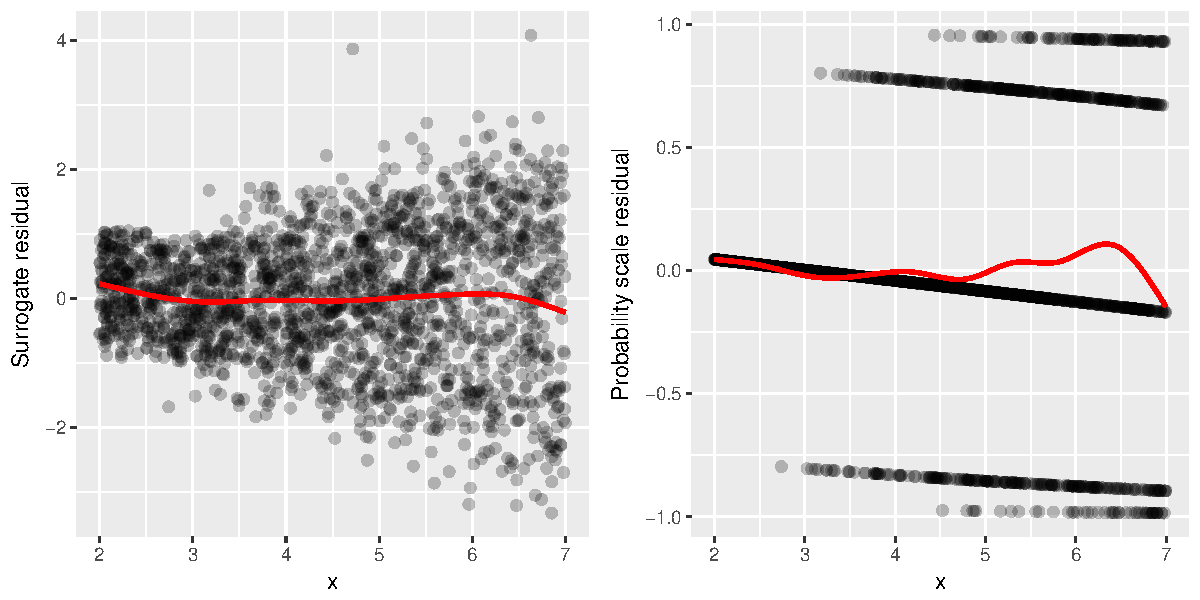
\includegraphics[width=1\textwidth]{heteroscedasticity}
  \caption{Residual vs. covariate plots for the simulated data. \textit{Left}: Surrogate residuals. \textit{Right}: SBS residuals.}
  \label{fig:heteroscedasticity}
\end{figure}

As outlined in Section~\ref{sec:jittering}, the jittering technique is broadly applicable to virtually all parametric and nonparametric models for ordinal responses. To illustrate, the code chunk below uses the \pkg{VGAM} package to fit a \dfn{vector generalized additive} model to the same data using a nonparametric smooth for $x$.
\begin{example}
library(VGAM)
fit.vgam <- vgam(y ~ s(x), family = cumulative(link = probit, parallel = TRUE),
                 data = df2)
\end{example}

To obtain a surrogate-based residual using the jittering technique, we can set \code{method = "jitter"} in the call to \code{resids} or \code{autoplot}. There is also the option \code{jitter.scale} which can be set to either \code{"probability"}, for jittering on the probability scale (the default), or \code{"response"}, for jittering on the response scale. In the code chunk below, we use the \code{autoplot} function to obtain residual-by-covariate plots using both types of jittering. The results, which are displayed in Figure~\ref{fig:heteroscedasticity2}, clearly indicate that the variance increases with increasing $x$.
\begin{example}
set.seed(103)  # for reproducibility
p1 <- autoplot(fit.vgam, what = "covariate", x = df2$x, method = "jitter",
               xlab = "x")
p2 <- autoplot(fit.vgam, what = "covariate", x = df2$x, method = "jitter",
               jitter.scale = "response", xlab = "x")
grid.arrange(p1, p2, ncol = 2)  # Figure ?
\end{example}

\begin{figure}[!htbp]
  \centering
  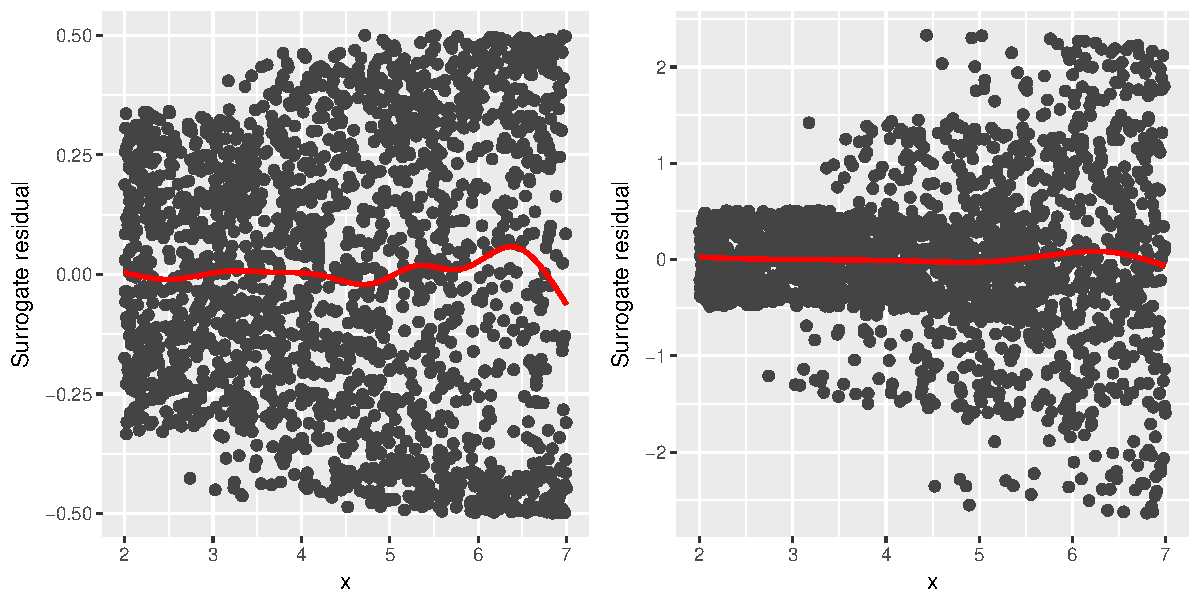
\includegraphics[width=1\textwidth]{heteroscedasticity2}
  \caption{Residual vs. covariate plots from a VGAM fit to the simulated data. \textit{Left}: Jittering on the probability scale (default). \textit{Right}: Jittering on the response scale.}
  \label{fig:heteroscedasticity2}
\end{figure}


%%%%%%%%%%%%%%%%%%%%%%%%%%%%%%%%%%%%%%%%%%%%%%%%%%%%%%%%%%%%%%%%%%%%%%%%%%%%%%%%
\subsection{Detecting a misspecified link function}
%%%%%%%%%%%%%%%%%%%%%%%%%%%%%%%%%%%%%%%%%%%%%%%%%%%%%%%%%%%%%%%%%%%%%%%%%%%%%%%%

For this example, we simulated $n = 2000$ observations from the following model
\begin{equation*}
  Pr\left(\mathcal{Y} \le j\right) = \Phi\left(\alpha_j + \beta_1 X + \beta_2 X ^ 2\right), \quad j = 1, 2, 3, 4
\end{equation*}
The data are available in the data frame \code{df3} within the package; see \code{?df3} for details.

below we fit a model with various link functions. For this model, however, the correct link function to use is the log-log link. From these models, we construct Q-Q plots of the residuals using $R = 100$ bootstrap replicates. The results are displayed in Figure~\ref{fig:link}.
\begin{example}
# Fit models with various link functions to the simulated data
fit.probit <- polr(y ~ x + I(x ^ 2), data = df3, method = "probit")
fit.logistic <- polr(y ~ x + I(x ^ 2), data = df3, method = "logistic")
fit.loglog <- polr(y ~ x + I(x ^ 2), data = df3, method = "loglog")  # correct link
fit.cloglog <- polr(y ~ x + I(x ^ 2), data = df3, method = "cloglog")

# Construct Q-Q plots of the surrogate residuals for each model
p1 <- autoplot(fit.probit, nsim = 100, what = "qq")
p2 <- autoplot(fit.logistic, nsim = 100, what = "qq")
p3 <- autoplot(fit.loglog, nsim = 100, what = "qq")
p4 <-  autoplot(fit.cloglog, nsim = 100, what = "qq")

# Figure ?
grid.arrange(p1, p2, p3, p4, ncol = 2)  # bottom left plot is correct model
\end{example}
From the Q-Q plots in Figure~\ref{fig:link}, it is clear the the model with the log-log link (which corresponds to gumbel errors in the latent variable formulation) is the most appropriate, while the other plots indicate deviations from the hypothesized model.

\begin{figure}[!htbp]
  \centering
  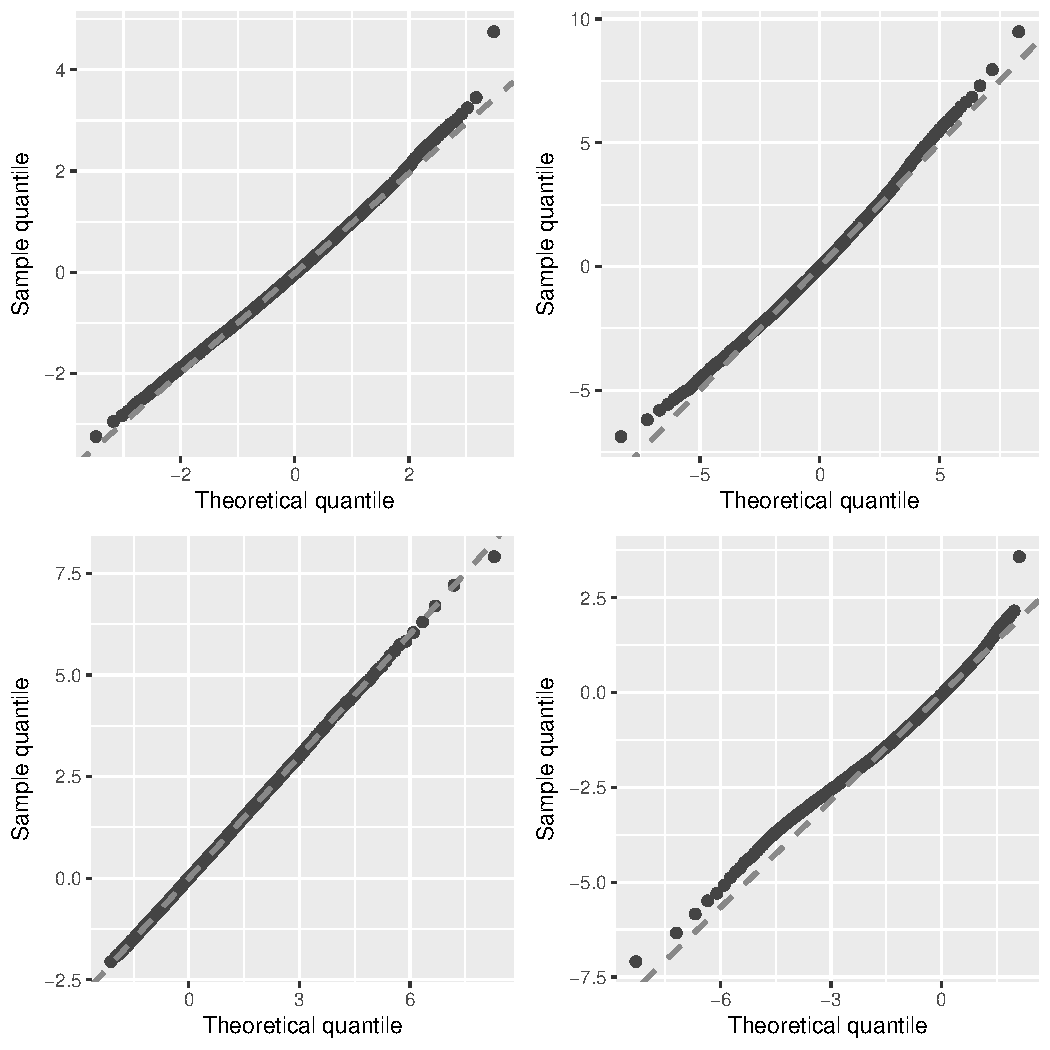
\includegraphics[width=0.7\textwidth]{link}
  \caption{Q-Q plots of the residuals for various cumulative link models fit to simulated data with gumbel errors. \textit{Top left}: A model with probit link. \textit{Top right}: A model with logit link. \textit{Bottom left}: A model with log-log link (i.e., the correct model). \textit{Bottom right}: A model with complementary log-log link.}  
  \label{fig:link}
\end{figure}

Alternatively, we could also use the surrogate residuals to make use of existing distance-based goodness-of-fit (GOF) tests; for example, the Kolmogorov-Smirnov distance. The \code{gof} function in the \pkg{sure} can be used to produce simulated $p$-values from such tests. 

Currently, the \code{gof} function supports three goodness-of-fit tests: the Kolmogorov-Smirnov test (\code{test = "ks"}), the Anderson-Darling test (\code{test = "ad"}), and the Cramer-Von Mises test (\code{test = "cvm"}). Below, we use the \code{gof} function to simulate $p$-values from the Anderson-Darling test for each of the four models; we also set \code{nsim} to 100 to produce smoother plots and reduce the sampling error induced by the surrogate procedure. The \code{plot} method is then used to display the empirical distribution function (EDF) of the simulated $p$-values. A good fit would imply uniformly distributed $p$-values; hence, the EDF would be relatively straight with a slope of one. The results, which are displayed in Figure~\ref{fig:gof}, agree with the Q-Q plots from Figure~\ref{fig:link} in that the log-log link is the most appropriate for these data. (\strong{Note} that the plotting method for \code{"gof"} objects uses base R graphics; hence, we can use the \code{par} function to set various graphical parameters.)
\begin{example}
# Figure ?
par(mfrow = c(2, 2), mar = c(2, 4, 2, 2) + 0.1) 
set.seed(8491)  # for reproducibility
plot(gof(fit.probit, nsim = 100, test = "ad"), main = "")
plot(gof(fit.logistic, nsim = 100, test = "ad"), main = "")
plot(gof(fit.loglog, nsim = 100, test = "ad"), main = "")
plot(gof(fit.cloglog, nsim = 100, test = "ad"), main = "")
\end{example}

\begin{figure}[!htbp]
  \centering
  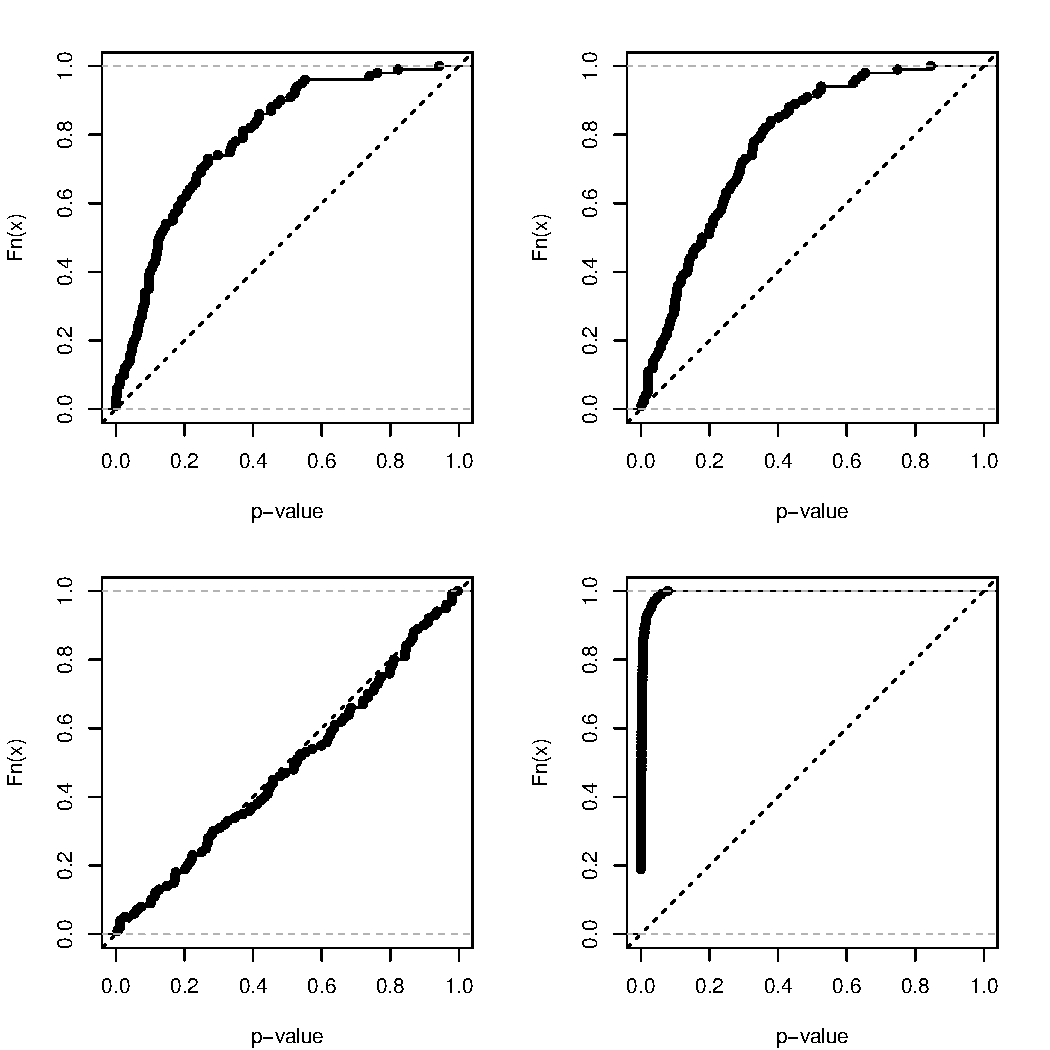
\includegraphics[width=0.7\textwidth]{gof}
  \caption{EDFs of the simulated $p$-values from an Anderson-Darling GOF test for various cumulative link models fit to simulated data with gumbel errors. \textit{Top left}: A model with probit link. \textit{Top right}: A model with logit link. \textit{Bottom left}: A model with log-log link (i.e., the correct model). \textit{Bottom right}: A model with complementary log-log link.}  
  \label{fig:gof}
\end{figure}


%%%%%%%%%%%%%%%%%%%%%%%%%%%%%%%%%%%%%%%%%%%%%%%%%%%%%%%%%%%%%%%%%%%%%%%%%%%%%%%%
\subsection{Checking the proportionality assumption}
%%%%%%%%%%%%%%%%%%%%%%%%%%%%%%%%%%%%%%%%%%%%%%%%%%%%%%%%%%%%%%%%%%%%%%%%%%%%%%%%

An important feature of the cumulative link model \eqref{eqn:clm} is the proportional odds assumption, which assumes that mean structure, $f\left(\boldsymbol{X}, \boldsymbol{\beta}\right)$, remains the same for each of the $J$ categories; for the logit case (see row one of Table~\ref{tab:common}), this is also referred to as the proportional odds assumption. \citet[pp. 334--335]{regression-harrell-2001} suggests computing each observation's contribution to the first derivative of the log likelihood function with respect to $\boldsymbol{\beta}$, average them within each of the $J$ categories, and examine any trends in the residual plots, but these plots can be difficult to interpret. Fortunately, it is relatively straightforward to use the simulated surrogate response values $S$ to check the proportionality assumption.

To illustrate, we generated 2000 observations from each of the following probit models
\begin{equation*}
  Pr\left(\mathcal{Y} \le j\right) = \Phi\left(\alpha_j + \beta_1 X\right), \quad j = 1, 2, 3, \quad \textrm{and} \quad Pr\left(\mathcal{Y} \le j\right) = \Phi\left(\alpha_j + \beta_2 X\right), \quad j = 4, 5, 6,
\end{equation*}
where $\alpha_1 = -1.5$, $\alpha_2 = 0$, $\alpha_3 = 1$, $\alpha_4 = 3$, $\beta_1 = 1$, and $\beta_2 = 1.5$. (The R code for generating the data can be made available upon request.) 

Checking the proportionality assumption here amounts to checking whether or not $\beta_1 - \beta_2 = 0$. As outlined in \citet{residuals-liu-2017}, we can generate surrogates $S_1 \sim \mathcal{N}\left(-\beta_1 X, 1\right)$ and $S_s \sim \mathcal{N}\left(-\beta_2 X, 1\right)$, both conditional on $X$. We then define the difference $D = S_2 - S_1$ which, conditional on $X$, follows a $\mathcal{N}\left(\left(\beta_1 - \beta_2\right) X, 1\right)$ distribution. If $\beta_1 - \beta_2 = 0$, then $D$ should be independent of $X$. This can be easily checked by plotting $D$ against $X$. Below, we use the \code{surrogate} function to generate the surrogate response values directly (as opposed to the residuals) and generate the $D$ vs. $X$ plot shown in Figure~\ref{fig:proportionality}.
\begin{example}
# Fit separate models (VGAM should already be loaded)
fit1 <- vglm(y ~ x, data = df4[1:2000, ], 
             cumulative(link = probit, parallel = TRUE))
fit2 <- update(fit1, data = df4[2001:4000, ])

# Generate surrogate response values
s1 <- surrogate(fit1)
s2 <- surrogate(fit2)

# Figure ?
ggplot(data.frame(D = s1 - s2, X = df4[1:2000, ]$x) , aes(x = X, y = D)) +
  geom_point() +
  geom_smooth(se = FALSE)
\end{example}
From Figure~\ref{fig:proportionality}, it is clear that $\beta_1 - \beta_2 \ne 0$; hence, the proportionality assumption does not hold.

\begin{figure}[!htbp]
  \centering
  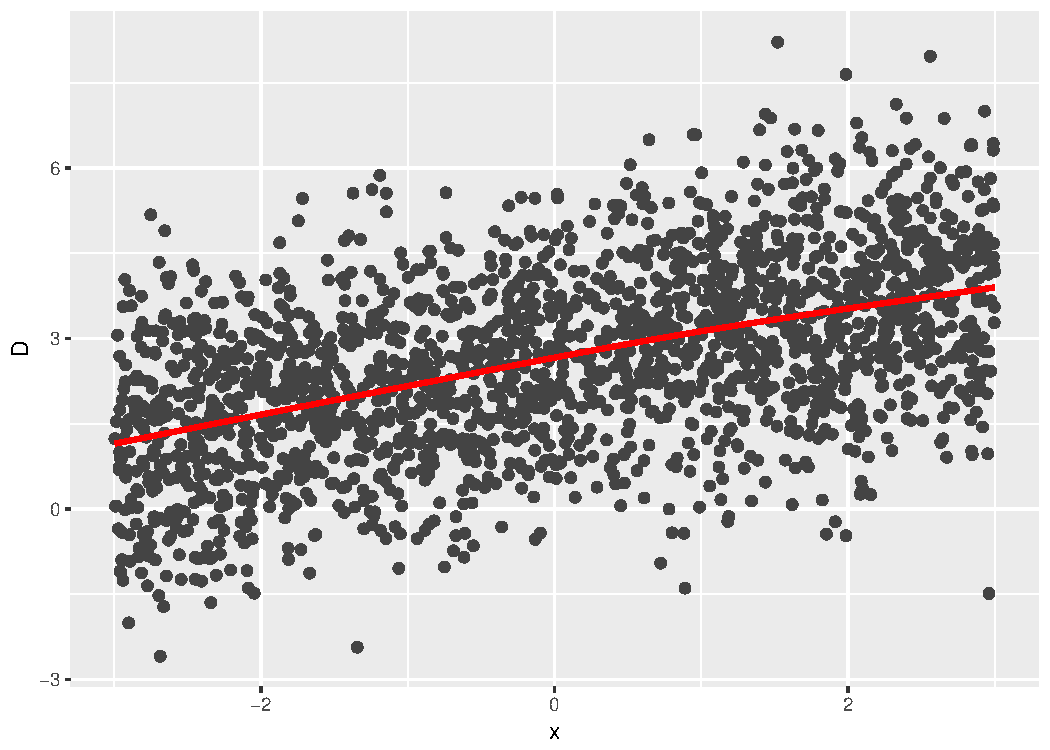
\includegraphics[width=0.7\textwidth]{proportionality}
  \caption{Scatterplot of $D = S_1 - S_2$ vs. $X$. A nonparametric smooth is represented by the red curve.}
  \label{fig:proportionality}
\end{figure}


% %%%%%%%%%%%%%%%%%%%%%%%%%%%%%%%%%%%%%%%%%%%%%%%%%%%%%%%%%%%%%%%%%%%%%%%%%%%%%%%%
% \section{Bitterness of wine}
% %%%%%%%%%%%%%%%%%%%%%%%%%%%%%%%%%%%%%%%%%%%%%%%%%%%%%%%%%%%%%%%%%%%%%%%%%%%%%%%%
% 
% \begin{example}
% library(ordinal)
% data(wine, package = "ordinal")
% wine.clm <- clm(rating ~ temp * contact, data = wine)  # default logit link
% \end{example}
% 
% \begin{example}
% set.seed(101)  # for reproducibility
% grid.arrange(
%   autoplot(wine.clm, nsim = 10, what = "qq"),
%   autoplot(wine.clm, nsim = 10, what = "fitted"),
%   autoplot(wine.clm, nsim = 10, what = "cov", x = wine$temp),
%   autoplot(wine.clm, nsim = 10, what = "cov", x = wine$contact),
%   ncol = 2
% )
% \end{example}
% 
% \begin{figure}[!htbp]
%   \centering
%   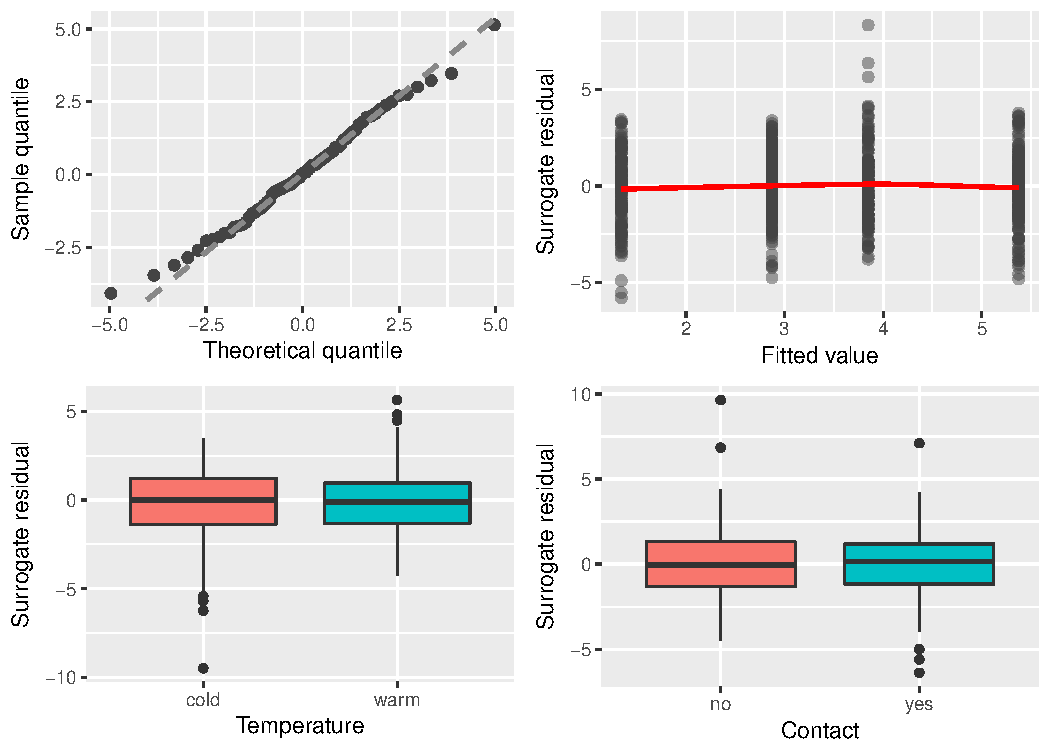
\includegraphics[width=1\textwidth]{wine}
%   \caption{Residual diagnostic plots for the quality of wine example.}
%   \label{fig:wine}
% \end{figure}
% 


%%%%%%%%%%%%%%%%%%%%%%%%%%%%%%%%%%%%%%%%%%%%%%%%%%%%%%%%%%%%%%%%%%%%%%%%%%%%%%%%
\section{Summary}
%%%%%%%%%%%%%%%%%%%%%%%%%%%%%%%%%%%%%%%%%%%%%%%%%%%%%%%%%%%%%%%%%%%%%%%%%%%%%%%%

In this paper, we have introduced the \pkg{sure} package which implements the surrogate approach to residuals for ordinal regression models described in \citet{residuals-liu-2017}. Using simulated data sets, we have illustrated the various properties of these residuals and how they can be used to check various assumptions in the ordinal regression model (e.g., heteroscedasticity, misspecified link functions, etc.) using continuous residuals which produce diagnostic plots not unlike those seen in ordinary linear regression. This offers a new way of performing typical diagnostic checks for ordinal regression models that are easily interpreted by the analyst. Furthermore, this new approach to constructing residuals for ordinal regression models is still under active development and new functionality will be added to \pkg{sure} accordingly in the future.



%%%%%%%%%%%%%%%%%%%%%%%%%%%%%%%%%%%%%%%%%%%%%%%%%%%%%%%%%%%%%%%%%%%%%%%%%%%%%%%%
\section{Acknowledgments}
%%%%%%%%%%%%%%%%%%%%%%%%%%%%%%%%%%%%%%%%%%%%%%%%%%%%%%%%%%%%%%%%%%%%%%%%%%%%%%%%

TBD.


\bibliography{greenwell-mccarthy-boehmke-liu}

\address{Brandon M. Greenwell\\
  Illumination Works\\
  6289 Commons Blvd\\
  Suite 120\\
  Beavercreek, OH 45431\\
  United States of America\\
  \email{greenwell.brandon@gmail.com}}

\address{Andrew McCarthy\\
  The Perduco Group\\
  3610 Pentagon Blvd\\
  Suite 110\\
  Beavercreek, OH 45431\\
  United States of America\\
  \email{andymc82000@yahoo.com}}

\address{Bradley C. Boehmke\\
  Air Force Institute of Technology\\
  2950 Hobson Way\\
  Wright-Patterson AFB, OH 45433\\
  United States of America\\
  \email{bradleyboehmke@gmail.com}}
  
\address{Dungang Liu\\
  University of Cincinnati\\
  2925 Campus Green Dr\\
  Cincinnati, OH 45221\\
  United States of America\\
  \email{dungang.liu@uc.edu}}
